\include{header}

\usepackage{macros}

\author{
\Large
Homework 2: Language modeling + count-based LMs \\ \Large+ preliminaries to neural networks 
}


\begin{document}

\maketitle 

\noindent\fbox{
    \parbox{\textwidth}{
        \textbf{Homework goals:} After completing this homework, you should be able to be comfortable with various foundational concepts related to our course.   
         Specifically, we hope you will gain the followings: 
        \begin{itemize}
            \item Get more comfortable with linear algebra, specifically gradients and Jacobians! 
            \item Gain a better grasp of count-based language models! 
            \item Get comfortable with activation functions such as the Softmax function!
            \item Know how to develop your own classifier! 
        \end{itemize}
    }
}

\vspace{0.5cm}

\noindent\textbf{How to hand in your written work:} Via MyClasses as before. 

\clearpage

\section{Concepts, intuitions and big picture}
% \subsection{Training Neural Nets}

\begin{enumerate}
    \item The $n$-gram models we've shown make the $n$-th order Markov assumption, i.e. that the distribution of words depends only on the previous $n - 1$ words. What properties of language will it not capture? Discuss (briefly) several distinct ways in which this assumption is false for natural language.\\
    \solution{The n-gram model does not capture some properties. This can be long range dependencies. For example in the sentence "The book I borrowed from the library was interesting" Since the subject book is connected to the adjective of the subject which is interesting. Small n would not recognize this. Another example is world knowledge and pragmatics meaning that the sentence requires external knowledge. For example "The capital of France is Paris" Relies on the facts that an n-gram model does not inherently possess.}
    \item  Follow-up to previous question: Despite the Markov assumption, $n$-gram models are remarkably good at predicting the next word. Discuss why this might be. What information is in the previous word(s) that makes these models perform so surprisingly well? In particular, what kinds of grammatical information do they capture?\\
    \solution{Some reasons the Markov assumption n-gram models does so well in next word prediction due to its local coherence and short range dependencies. Many words in natural language have strong dependencies on recent words or common phrases. Another reasons is its grammatical consistency. Using Part of speech constraints allows it to learn that a determiner like "the" is likely followed by a noun like cat rather than a verb.} 
    \item Explain how are perplexity and cross-entropy loss related? \\ 
    \solution{The cross entropy loss measures how well the model predicted probability distribution aligns with the true distribution. The perplexity represents the effective number of choices the model considers for each word. The lower the perplexity indicates a better model as it assigns higher probabilities to correct words.}
    \item For a vocabulary of $|V|$ words, what would you expect perplexity to be if your model predictions were completely random? Compute the corresponding cross-entropy loss for $|V| = 2000$ and $|V| = 10000$, and keep this in mind as a baseline.\\
    \solution{If it was completely random it assigns a uniform probability to each word in the vocabulary. perplexity is defined as: $$2^H(p,q)$$   where the cross entropy loss H(p,q) is $$= -summation abs(V) over i=1 p(w_i) log_2 q(w_i)$$. Since the model is making random predictions the true distribution is $$=-log_2 1/abs(V) =log_2 abs(V)$$. Thus the perplexity = 2} 

    \item Which of these are reasons for the recent wave of neural networks taking off? (check the options that apply.) \\ 
        \hspace{1cm}\choice{\checkmark} We have access to a lot more computational power.\\
        \hspace{1cm}\choice{} Neural Networks are a brand new field.\\
        \hspace{1cm}\choice{\checkmark} We have access to a lot more data.\\
        \hspace{1cm}\choice{\checkmark} There has been significant improvements in benchmarks in speech recognition and NLP.\\
        \solution{}
    \item What does a neuron compute? \\ 
        \hspace{1cm}\choice{} A neuron computes an activation function followed by a linear function ($z = Wx + b$)\\
        \hspace{1cm}\choice{\checkmark} A neuron computes a linear function ($z = Wx + b$) followed by an activation function.\\
        \hspace{1cm}\choice{} A neuron computes a function $g$ that scales the input $x$ linearly ($Wx + b$).\\
        \hspace{1cm}\choice{} A neuron computes the mean of all features before applying the output to an activation function.\\
        \solution{}

    \item  What is the point of applying a Softmax function to the logits output by a sequence classification model? \\ 
        \hspace{1cm}\choice{} It softens the logits so that they're more reliable. \\ 
        \hspace{1cm}\choice{} It applies a lower and upper bound so that they're understandable. \\ 
        \hspace{1cm}\choice{\checkmark} The total sum of the output is then 1, resulting in a possible probabilistic interpretation.\\
        \solution{}
    
\end{enumerate}

\clearpage

\section{Linear Algebra Recap}
\subsection{Gradients}
Consider the following scalar-valued function: 
$$
    f(x, y, z) = x^2y + \text{sin}(z+6y). 
$$

\begin{enumerate}
    \item Compute partial derivatives with respect to $x$, $y$ and $z$. \\
    \solution{With respect to x: $theta f/theta x =2xy$, with respect to y: $Theta f/ theta y =x^2+6cos(z+6y)$, with respect to z: $theta f/ theta z = cos(z+6y)$}
    
    \item We can consider $f$ to be a function that takes a vector $\theta \in \reals^3$ as input, where $\theta = [x, y, z]^\top$. 
    Write the gradient as a vector and evaluate it at $\theta = [3, \pi/2, 0]^\top$.\\
    \solution{$\textbf{delata f(3,pi/2,0)} = 
\begin{bmatrix}
3pi\\  
3\\ 
-1 
\end{bmatrix}$}
\end{enumerate}


%%%%%%%%%%%%%%%%%%%%%




\subsection{Gradients of vectors}

Let $\mathbf{x}, \mathbf{c} \in \reals^n$ and $\mathbf{A} \in \reals^{n \times n}$. 
For the following parts, before taking any derivatives, identify what the
derivative looks like (is it a scalar, vector, or matrix?) and how we calculate each term in the derivative. Then carefully solve for an arbitrary entry of the derivative, then stack/arrange all of them to get the final
result. 

\begin{itemize}
    \item Show that $\frac{\partial }{ \partial \mathbf{x} } \left( \mathbf{x}^\top \mathbf{c}  \right) = \mathbf{c}^\top$.\\
    \solution{Step 1: identify the shape. X is an n-dimensional vector, c is an n- dimensional vector, $$x^Tc$$ is a scalar, the derivative should be a row vector of size 1 x n. Step 2 compute an entry. Let $$x_i$$ be the i-th component of x. Differentiating with respect to $$x_i$$ . Stacking these creates a row vector.}
    \item Show that $\frac{\partial }{ \partial \mathbf{x} } \left( \norm{\mathbf{x}}^2_2 \right) = 2\mathbf{x}^\top$.\\
    \solution{We identify the shape $$||x||^2_2=x^Tx$$, which is a scalar. By expanding the norm with $$\sum^n_\text{i=1} x^2_i$$ . with respect to $$x_i$$  the answer is $$2x_i$$  which stacking these into a row vector is $$2x^T$$ }
    \item Show that $$\frac{\partial }{ \partial \mathbf{x} } \left( \mathbf{A} \mathbf{x} \right) = \mathbf{A}$$.\\
    \solution{We identify the shape Ax is an n-dimensional vector, the derivative should be an n x n matrix. Step 2 we compute the j-th entry of Ax is $$\sum^ n_\text{i=1}  A_jiX_i$$ . with respect to $$x_i$$ is $$A_ji$$ . which can be assembled since each row of the derivative corresponds to a row of A we obtain A.}
    \item Show that $\frac{\partial }{ \partial \mathbf{x} } \left( \mathbf{x}^\top \mathbf{A}  \mathbf{x} \right) = \mathbf{x}^\top (\mathbf{A} + \mathbf{A}^\top)$.\\
    \solution{We identify the shape $$x^\text{TAx}$$ is a scalar, the derivative should be a row vector of size 1 x n. Step two we expand the quadratic form to be $$=\sum_\text{i=1}^n \sum_\text{j=1}^n  x_iA_ijX_j$$. rewriting this gives us $$x^T(A+A^T)$$}
\end{itemize}

\paragraph{Note:}The above equations follow the \href{https://en.wikipedia.org/wiki/Matrix_calculus#Layout_conventions}{numerator layout} notation which is commonly following in linear algebra, but there are alternative notational conventions as well. 

%%%%%%%%%%%

\subsection{Jacobian}
Consider the following vector function from $\reals^3$ to $\reals^3$: 
$$
    \mathbf{f}(\boldsymbol{\theta} = [x_1, x_2, x_3]) = 
    \begin{cases}
        \text{sin}(x_1x_2x_3) \\
        \text{cos}(x_2 + x_3) \\
        \exp(-\frac{1}{2}x_3^2) \\
    \end{cases}
$$

\begin{enumerate}
    \item What is the Jacobian matrix\footnote{\url{https://en.wikipedia.org/wiki/Jacobian_matrix_and_determinant}} of $\mathbf{f}(\boldsymbol{\theta})$?\\
    \solution{\[
J_{\mathbf{f}}(\boldsymbol{\theta}) =
\begin{bmatrix}
x_2 x_3 \cos(x_1 x_2 x_3) & x_1 x_3 \cos(x_1 x_2 x_3) & x_1 x_2 \cos(x_1 x_2 x_3) \\
0 & -\sin(x_2 + x_3) & -\sin(x_2 + x_3) \\
0 & 0 & -x_3 e^{-\frac{1}{2}x_3^2}
\end{bmatrix}
\]}
    
    \item Evaluate the Jacobian matrix of $\mathbf{f}(\boldsymbol{\theta})$ at 
    $\boldsymbol{\theta} = [1, \pi, 0]$.\\
    \solution{\[
J_{\mathbf{f}}(1, \pi, 0) =
\begin{bmatrix}
0 & 0 & \pi \\
0 & 0 & 0 \\
0 & 0 & 0
\end{bmatrix}
\]}
\end{enumerate}

\clearpage


\section{$n$-gram Language Models}
\subsection{A toy $n$-gram language model}

Consider the following vocabulary, $V= \{\tt BOS, EOS, who, framed, roger, rabbit, the\}$ where \texttt{BOS} is the dummy token indicating the beginning of a sentence, and \texttt{EOS} indicates the end of a sentence. Consider the following training data:

\noindent\fbox{%
    \parbox{0.5\textwidth}{%
\noindent
\texttt{BOS who EOS \\ 
BOS who framed roger EOS \\ 
BOS roger rabbit EOS \\ 
BOS who framed roger rabbit EOS \\ 
BOS roger framed who EOS \\ 
BOS who framed the rabbit EOS \\
}}}

\begin{enumerate}
    \item Compute the following probabilities: $P(\texttt{rabbit})$, $P(\texttt{rabbit}|\texttt{roger})$, $P(\texttt{EOS}|\texttt{rabbit})$.\\
    \solution{We must compute the word count. This is 19 total words. To compute P(rabbit) we must do count(rabbit)/total words. This is 2/19. Then we compute P(rabbit|roger). We do this by dividing count(roger rabbit) over count(roger) this is 2/3. Lastly to find P(EOS|rabbit we must do count(rabbit EOS)/count(rabbit) which is 2/2 or 1}

    \item Briefly  explain what the sparsity problem is in $n$-gram language models? \\
    \solution{The sparsity problem happens because real world language models have a vast vocabulary  and many possible word sequences but any given dataset only contains a small fraction of them. This means many sequences will gave zero probability, increasing n leads to exponentially more possible sequences and rare or unseen words result in zero probability.}
\end{enumerate}



\clearpage

\section{Challenges of linear classifiers of sentences}
A simple way to compute a representation for a phrase $s$ is to add up the representations of the words in that phrase: $\text{repr}(s) = \sum_{w \in s} v_w$, 
where $w \in s$ are the word in  $s$ and $v_w \in \reals^d$ is the embedding for word $w$. 

\begin{enumerate}
    \item  Now, consider sentiment analysis on a phrase in which the predicted sentiments are 
        $$ f(s; \theta) = \theta \cdot \text{repr}(s), $$
        for some choice of parameters $\theta$. 
        Note that here $\theta  \in \reals^d$ and ``$\cdot$'' is the ``dot-product''. 
        Prove that in such a model, the following inequality cannot hold for any choice of $\theta$ and word embeddings: 
        \begin{align*}
            f(\texttt{good}; \theta)  > f(\texttt{not good}; \theta)    \\ 
            f(\texttt{bad}; \theta)  < f(\texttt{not bad}; \theta)
        \end{align*}
        Thereby, showing the inadequacy of this model in capturing negations.\footnote{Question credit: ``Introduction to Natural Language Processing'' by J. Eisenstein.} \\ 
    \solution{Using the function above and creating the dot product as $$\Theta * \sum_{wEs}v_w $$ For a phrase like "not good" the representation is $$repr\text{(not good)}=v_\text{not} +v_\text{good}$$ and similarly for "not bad". The predictions for the phrase become $$f(good;\theta)=\theta * v_\text{good}$$ $$f(\text{not good};\theta)=\theta*(v_\text{not}+v_\text{good})$$ and similarly for bad and not bad. We can then rewrite these inequalities as $$\theta*v_\text{good}>\theta*(v_\text{not}+v_\text{good})$$ $$\theta*v_\text{bad}>\theta*(v_\text{not}+v_\text{bad})$$ This can be rearranged to be $$0>\theta*v_\text{not}$$ $$0<\theta*v_\text{not}$$ These are contradictory because they state the $$\theta * v_\text{not}$$ must be both positive and negative at the same time.} 
   
    \item  Consider a slight modification to the previous predictive model: 
        $$ 
            f(s; \theta) = \theta \cdot \text{ReLU}\big( \text{repr}(s) \big), 
        $$
        where ReLU (rectified linear function) is defined as: 
        $$
            \text{ReLU}(x) = 
            \begin{cases}
                x & \text{ if } x \geq 0  \\ 
                0 & \text{ if } x < 0.
            \end{cases}
        $$
        Given this choice of predictive function, show that it is possible to satisfy the above inequalities for some choice of $\theta$. 
        \textbf{Hint:} Show there exists parameters $\theta$ and word embeddings $v_\texttt{good}$, $v_\texttt{bad}$ and $v_\texttt{not}$ that the inequalities are satisfied. \\ 
    \solution{Lets assume the vectors representations as: $$v_\text{good}=[1,1], v_\text{bad}=[-1,-1], v_\text{not}=[-2,-2]$$ First we compute the phrase $$repr(good)=[1,1]$$ $$repr(\text{not good)}=v_\text{not}+v_\text{good}=[-1,-1]$$ $$repr(bad)=[-1,-1]$$ $$repr(\text{not bad)}=v_\text{not}+v_\text{bad}=[-3,-3]$$
Now we can apply ReLU which shows
$$ReLU(good)=[1,1], ReLU(\text{not good)=[0,0]}),ReLU(bad)=[0,0], ReLU(\text{not bad})=[0,0]$$
now choosing $$\theta=[1,1]$$ $$f(good;\theta)=[1,1]*[1,1]=2$$
while the rest of the combinations equal 0. Thus the inequalities $$f(good)>f(\text{not good}), f(bad)<f(\text{not bad})$$}

\item Given the above result, explain (in 1-2 sentence) why the use of neural networks (which have more complexity than linear models)
    \\
    \solution{Neural networks introduce non-linearity by activating functions like ReLU and allowing the model to transform the representation in a way that allows for complex dependencies such as negation. Unlike a linear model a neural network can learn contextual meaning by changing words.}
\end{enumerate}


% \newpage %%%%%%%%%%%%%%%%%%%%%%%%%%%%%%%%%%%%%%%%%%%%%%%%%%%%%%%%%%%%%%%%%%%%%%%%%%%%%%%%%%

\section{Softmax function}
\label{sec:softmax}
Remember  the Softmax functions from the class: 
$$
    \text{Softmax: } \sigma(\mathbf{z}) \triangleq [\sigma(\mathbf{z})_1, \hdots, \sigma(\mathbf{z})_K] \; \text{s.t.} \;  \sigma(\mathbf{z})_i = \frac{e^{z_i}}{\sum_{j=1}^K e^{z_j}} \ \ \text{ for } i = 1, \dotsc, K \text{ and } \mathbf{z} = (z_1, \dotsc, z_K)
$$

\begin{enumerate}
    \item  Prove that Softmax is invariant to constant offsets in the input, i.e., for any input vector \label{subsec:5.1}
    $\mathbf{z}$ and any constant $c$,
    $$
        \sigma(\mathbf{z}) = \sigma(\mathbf{z} + c) 
    $$
    \textbf{Pro tip: } We make use of this property in practice to increase the numerical stability of our models. 
    Specifically, using  $c = - \max_{i \in \set{1 ... K}} z_i$, i.e. subtracting its maximum element from all elements of $\mathbf{z}$ would prevent numerical instability  due to large values. \\
    \solution{We must show that for any constant the softmax function works. $$
        \sigma(\mathbf{z}) = \sigma(\mathbf{z} + c) 
    $$ We can start with the definition of softmax: $$\sigma (z)_i=e^\text{zi}/\sum_\text{j=1}^Ke^\text{zj}$$ Now define a new input vector z+c where every element is shifted by a constant
$$\sigma (z+c)_i=e^\text{zi+c}/\sum_\text{j=1}^Ke^\text{zj+c}$$  Factor out the $$e^c$$  from both the numerator and denominator. Since $$e^c$$  is a common factor both cancel out. leaving us with $$\sigma (z+c)_i=e^\text{zi}/\sum_\text{j=1}^Ke^\text{zj}$$ which is exactly $$\sigma(z)_i$$  proving the softmax is invariant to constant shifts in z. }
    
    \item Softmax maintains the relative order of the elements in $\mathbf{z}$. In particular, show that the largest index is intact after applying Softmax: 
    $$
        \argmax_{i \in \set{1 ... K}} z_i =  \argmax_{i \in \set{1 ... K}}  \sigma(\mathbf{z})_i
    $$
    \solution{Using the definition of softmax $$\sigma (z)_i=e^\text{zi}/\sum_\text{j=1}^Ke^\text{zj}$$ Since the denominator is a constant for all i, the softmax function preserves the ranking of $$e^\text{zi}$$. The exponential function is monotonically increasing, meaning that if $$z_a>z_b \text{then } e^za>e^zb$$, and thus $$\sigma(z)_a>\sigma(z)_b$$. Therefore the index of the max value in z is the same as the index of the max values in sigma(z).}
    \item Define the Sigmoid function as follows: 
    $$
        \text{Sigmoid: } S(x) \triangleq \frac{1}{1 + e^{-x}} = \frac{e^x}{e^x + 1}=1-S(-x). 
    $$
    Prove that Softmax is equivalent to the Sigmoid functions when the number of possible labels is two: $K=2$. Specifically: 
    $$ \sigma_1([z_1, z_2]) = S(z_1 - z_2) $$
    \\
    \solution{By dividing both the numerator and denominator by $$e^z2$$: $$\sigma(|z_1,z_2|)=\frac{\frac{e^\text{z1}}{e^\text{z2}}}{\frac{e^\text{z1}}{e^\text{z2}}+1}$$ since $$e^z1/e^z2 = e^x1-x2$$ , we can rewrite it as $$\sigma_1(|z_1,z_2|)=\frac{e^\text{z1-z2}}{e^\text{z1-z2}+1}$$ which is the same as out Sigmoid function of $$S(z_1-z_2)$$  Thus we proved $$\sigma_1(|z_1,z_2|)=S(z_1,z_2)$$ This shows the sofmax generalized the sigmoid function when K=2.}
    
   
\end{enumerate}

\newpage
    



\section{Programming}
In this programming homework, we will
\begin{itemize}
    \item build a simple count-based (n-gram) language model.
    \item implement your own gradient descent optimization for the classifier you built in homework 1.
\end{itemize}


\noindent \paragraph{Skeleton Code and Structure:}
The code base for this homework can be found at MyClasses/Files under the \texttt{hw2} directory. Your task is to fill in the missing parts in the skeleton code, following the requirements, guidance, and tips provided in this pdf and the comments in the corresponding .py files.
The code base has the following structure:
\begin{itemize}
    \item \texttt{ngram\_lm.py} implements a n-gram language model on a subset of Wikipedia. 
    \item \texttt{gradient\_descent.py} reuse the sentiment classifier on movie reviews you implemented in homework 1, with additional requirements to implement manual softmax, cross-entropy loss, and gradient updates.
    \item \texttt{main.py} provides the entry point to run your implementations in both \texttt{ngram\_lm.py} and \texttt{backprop.py}.
    \item \texttt{hw2.md} provides instructions on how to setup the environment and run each part of the homework in \texttt{main.py}
\end{itemize}


\noindent \todo{} ---
Your tasks include
1) generate plots and/or write short answers based on the results of running the code; 2) fill in the blanks in the skeleton to complete the code. We will explicitly mark these plotting, written answer, and filling-in-the-blank tasks as \todo{} in the following descriptions, as well as a \textcolor{blue}{\texttt{\textbf{\#~TODO}}} at the corresponding blank in the code. \\

\noindent \todo{} (Copy from your HW1). We are reusing most of the \texttt{model.py} from homework 1 as the starting point for the \texttt{gradient.py} - you will see in the skeleton that they look very similar. Moreover, in order to make the skeleton complete, for all the \textcolor{blue}{\texttt{\textbf{\#~TODO (Copy from your HW1)}}}, please fill in the blank below them by copying and pasting the corresponding implementations you wrote for homework 1 (i.e. the corresponding \textcolor{blue}{\texttt{\textbf{\#~TODO}}} in homework 1.)

\noindent \paragraph{Submission:} Your submission should contain two parts: 1) plots and short answers under the corresponding questions below; and 2) your completion of the skeleton code base, in a \texttt{.zip} file

\subsection{Count-based LMs}
\label{subsubsec:count-based lms}
In the lecture, we have learned language modeling as building probabilistic distribution (marginal and joint) over language. Moreover, we can estimate such distributions (e.g. $\Pr(X_t|X1, \cdots, X_{t-1})$) by \textit{counting}. For example $$\Pr(\textrm{mat} | \textrm{the cat sat on the}) \approx \frac{\textrm{count}(\textrm{"the cat sat on the mat"})}{\textrm{count}(\textrm{"the cat sat on the"})} $$
We are going to implement such a count-based LM, i.e. n-gram language model.

\subsubsection{Data Loading}
We will use (a subset of) the \href{https://huggingface.co/datasets/wikitext}{WikiText} dataset for building the n-gram LM. The WikiText language modeling dataset is a collection of over 100 million tokens extracted from the set of verified Good and Featured articles on Wikipedia. 
Spend a few minutes reading a few examples on Huggingface to get a better sense of what this dataset looks like. We will use Huggingface's datasets library to download this dataset locally. For efficiency, we only use the first $1\textrm{e}5$ training samples to create our LM.\\\

\noindent Read the \texttt{load\_data} function in \texttt{ngram\_lm.py} for how we obtain the data.

\subsubsection{Preprocessing: Sentence Split and Tokenization}
As you have seen, each data sample consists of a Wikipedia paragraph. To perform our n-gram counting, we need first split each paragraph into sentences \footnote{we count n-gram status within sentence boundary} and then each sentence into a sequence of tokens (i.e. \textit{tokenization} that we introduced in homework 1).
In particular, we will use \href{https://aclanthology.org/W07-0733/}{an algorithm} by Philipp Koehn for sentence splitting; and use a \textit{sub-word tokenizer} for tokenization. For now, we are using an existing sub-word tokenizer of an existing model from the Huggingface library, but in the future, we will also build our own tokenizer.

A \textit{Sub-word tokenizer} which, as it should be clear from the name, splits each sentence into units smaller than words, based on their frequency. For example, the word "Potentials" is broken into four sub-words: `Po', '\#\#ten', '\#\#tial', '\#\#s'`, where `\#\#` is a special symbol indicating that the sub-word is in the middle of a word.


Sub-word tokenization might initially seem like a bad idea since we are breaking up the word. But it brings it several benefits.
\begin{itemize}
    \item Handling Out-of-Vocabulary (OOV) words: Sub-word tokenization allows the representation of rare or unseen words as a combination of sub-words or tokens that have been seen in the training data, thus reducing the OOV problem.
    \item Improved vocabulary size: It allows for a more compact vocabulary size, reducing the size of the language model, and increasing its efficiency.
    \item Better language model performance: Sub-word tokenization results in a better representation of morphologically rich languages, where words are formed by combining roots and affixes, leading to improved language model performance.
    \item Cross-lingual compatibility: Sub-word tokenization is language-agnostic, and models trained on sub-word tokens from one language can be applied to other languages, improving cross-lingual compatibility.
    
\end{itemize}

How are sub-tokenizers built? We will delve into that in a few weeks! For now, we will just use them!
\\\\
\noindent Read the \texttt{sentence\_split\_and\_tokenize\_demo} for how exactly an \texttt{wikitext} paragraph is converted into sentences and then tokens.

\subsubsection{Build the N-gram LM: Let's Count!}
\noindent\todo{}: read the \texttt{create\_ngrams} function which iteratively processes each paragraph and counts the n-gram statistics, and completes the following lines under three \textcolor{blue}{\texttt{\textbf{\#~TODO}}}s:
\begin{itemize}
    \item tokenize the words in the sentence: that takes in a \texttt{sentence} and convert it into \texttt{tokens} as a list of tokens with the tokenizer. \\
    \textbf{Hint}: check out how to do tokenization in sentence\_split\_and\_tokenize\_demo
    \item count n-gram statistics over each list of tokens, record them in
    \begin{itemize}
        \item \texttt{ngrams}: the \texttt{Counter} for n-grams count
        \item \texttt{ngram\_context}: the \texttt{Counter} for context (i.e. (n-1)-grams) 
        count
        \item \texttt{next\_word\_candidates}: the \texttt{Dictionary} that keeps track of all possible candidate next tokens given the context, i.e. all tokens that, concatenated with the (n-1)-gram context, constitutes an n-gram that exists in the data. 
    \end{itemize}
    for all the \texttt{Counter} and \texttt{Dictionary}, use \texttt{tuple} of n-gram or (n-1)-gram tokens as the keys. \\
    \textbf{Hint}: also check the corresponding comments in the code for specific requirements
    \item computes the estimated probability of the next word (token) given the context. \\\textbf{Hint}: use the formula in \autoref{subsubsec:count-based lms}, and also the corresponding comments in the code
\end{itemize}
Finally, the \texttt{next\_word\_pred} returned from the \texttt{create\_ngrams}, will record for each (n-1) gram context, the most probable next word continuation. For this homework, we will set $n=3$ so that to build a \textit{trigram} language model.

\subsubsection{Visualize the N-gram distribution}
\todo{}: Complete the \texttt{plot\_next\_word\_prob} function in \texttt{ngram\_lm.py}, and run \texttt{run\_ngram} in \texttt{main.py} to plot the top-10 most probable next token given an input context. Paste the two plots for the two given contexts (provided in \texttt{run\_ngram}), and describe in 2-3 sentences your findings. \\
\textbf{Hints}:
\begin{itemize}
    \item you can check out \href{https://www.geeksforgeeks.org/bar-plot-in-matplotlib/}{this tutorial} about how to plot bar chart with \href{https://matplotlib.org/stable/api/_as_gen/matplotlib.pyplot.bar.html}{matplotlib}.
    \item read the comments in the code carefully for more info about the input.
\end{itemize}
\noindent {\color{red}{your plots and answer:}}\\
%uncommment the following lines to add your figures
%\begin{figure}[h] 
%    \centering
%    \subfloat[top 10 next words of "move to"]{
%        \includegraphics[width=0.45\textwidth]{}
%        }
%    \hfill
%    \subfloat[top 10 next words of "the news"]{
%        \includegraphics[width=0.45\textwidth]{}
%        \label{fig:b}
%        }
%    \caption{The probabilities of top 10 next words of two bi-gram contexts}
%\end{figure}

\noindent\solution{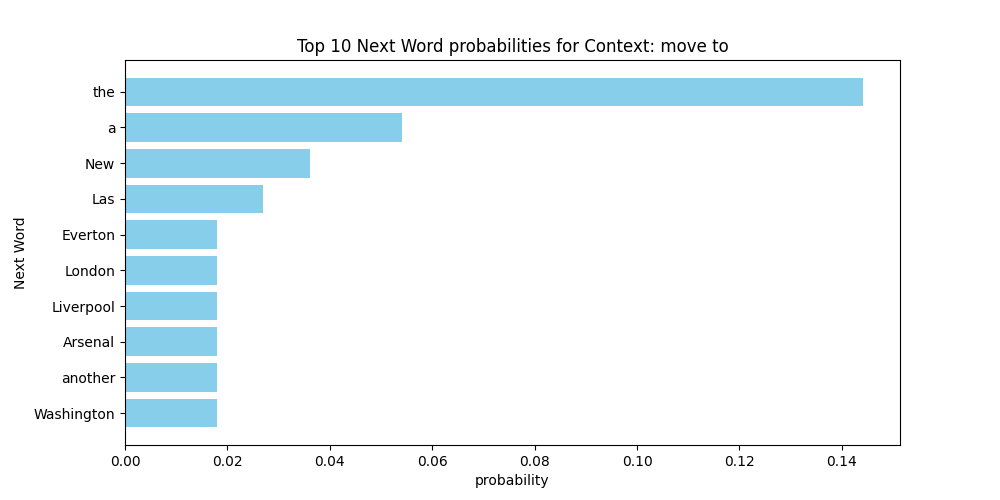
\includegraphics[width=\textwidth]{ngram_context1.png} 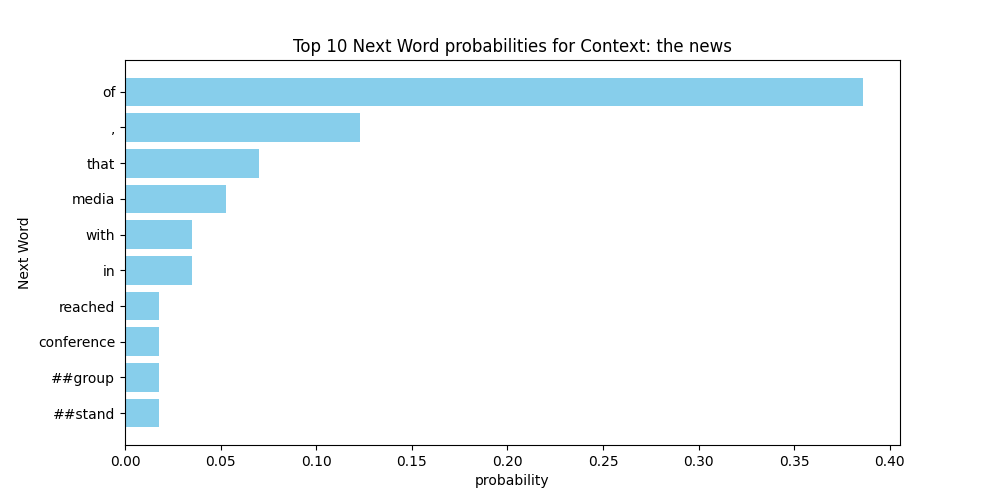
\includegraphics[width=\textwidth]{ngram_context2.png} Based on the two graphs we can see that in the move to graph that the is by far the dominate word. Most likely do to its conjunction nature and being very common in our language. Similarly in the news graph we see of being very common mostly because when hearing the news typically they start by giving context of what your watching.}

\subsubsection{Generation: Sample from the LM}
Now that we have built our LM, given any prefix\footnote{in our case of trigram LM, we require the prefix to have $\geq2$ tokens}, we can sample from the LM to generate a full completion. Specifically, at each timestamp, we take the last (n-1) tokens from the prefix as the context and query our LM to get the most probable next token, append it to the prefix, and continue until we sample the stop token our the maximum length is reached. 

This sampling procedure is called greedy decoding, as we take the most probable next token each step, there are a few other sampling strategies like beam search \citep{meisteretal2020beam}, top-k, and top-p sampling \citep{holtzman2019curious}. Similarly, we will get to them soon.
\\\\
\noindent Read the \texttt{generate\_text} function in \texttt{ngram\_lm.py} for details of the generation process described above.
\\\\
\noindent \todo{}: Run \texttt{run\_ngram} in \texttt{main.py} and paste the completion of the two given prefixes (provided in \texttt{run\_ngram}), and describe in 2-3 sentences your findings.
\\
\solution{\\Completion 1: According to the report\\
Completion 2: The president of the association\\
Findings: }

\subsection{Optimizing the Sentiment Classifier with (Stochastic) Gradient Descent}
In the second part of this programming homework, we will revisit the sentiment classifier we built in the last homework. Instead of relying on the PyTorch built-in loss functions, gradient calculations, and weights optimization, we will delve into them and implement our own version!

\subsubsection{Reuse Your HW1 Implementation}
\todo{} (Copy from your HW1): for all the \textcolor{blue}{\texttt{\textbf{\#~TODO (Copy from your HW1)}}} in \texttt{gradient\_descent.py}, please fill in the blank below them by copying and pasting the corresponding implementations you wrote for homework 1 (i.e. the corresponding \textcolor{blue}{\texttt{\textbf{\#~TODO}}} in the \texttt{model.py} in homework 1).

\subsubsection{Softmax Function}
Remember the \href{https://pytorch.org/docs/stable/generated/torch.nn.CrossEntropyLoss.html}{nn.CrossEntropyLoss} we used in homework 1, it can be further decomposed into that 1) normalize the real-value scores of each class (e.g. the logits) into a probability distribution
using softmax function, and calculate the cross entropy loss of this probability distribution against the ground truth binary distribution (In practice, PyTorch instead provides the combination of \href{https://pytorch.org/docs/stable/generated/torch.nn.LogSoftmax.html#torch.nn.LogSoftmax}{LogSoftmax} with \href{https://pytorch.org/docs/stable/generated/torch.nn.NLLLoss.html#torch.nn.NLLLoss}{negative log likelihood loss}).  We will first implement the softmax function, which you have been familiar with in the lecture, and \autoref{sec:softmax}.
\\\\
\noindent \todo{}: Complete the \texttt{softmax} function of the \texttt{SentimentClassifier} class in \texttt{gradient\_descent.py}. Note: you must implement the optimized for numerical stability version described in the \textbf{Pro tip} in \autoref{subsec:5.1} of \autoref{sec:softmax}.
\\
\noindent \textbf{Hint}: check the comments in the code for specific input-output requirements.
\\
A correct implementation should pass the \texttt{test\_softmax} in \texttt{gradient\_descent.py}.
\\\\
\noindent With the softmax function, we turn our neural network into a classifier that assigns a probability distribution over the 2 sentiment classes. Specifically, denoting our input feature vector as $\mathbf{x}$, the \texttt{nn.Linear} layer transforms $\mathbf{x}$ into a \textbf{logit score} vector $\mathbf{z}$ using a weight matrix $W$ and a bias vector $\mathbf{b}$:

$$
    \mathbf{z} = \mathbf{x} W + \mathbf{b}
$$

This logit score has one element per class, so the weight matrix must have a size $(d, c)$, where $c$ is the number of classes (output labels) and $d$ is the number of dimensions of the input space (features). The bias vector has $c$ elements (one per class).

The logit score is turned into probabilities using the \textbf{softmax}  operator:

$$
    \hat{y}_j = \Pr(\text{class = j}) = \frac{\exp(z_j)}{\sum_k \exp(z_k)}
$$


\subsubsection{Gradients on Cross Entropy Loss}
We will start by defining an objective function that defines "goodness" for our classifier.
A common choice for classification is \href{https://en.wikipedia.org/wiki/Cross_entropy}{categorical cross-entropy loss} or negative log-likelihood.

A discussion or derivation of cross-entropy loss is beyond the scope of this class but a good introduction to it can be \href{https://rdipietro.github.io/friendly-intro-to-cross-entropy-loss/}{found here}. A discussion of what makes it superior to MSE for classification can be \href{https://jamesmccaffrey.wordpress.com/2013/11/05/why-you-should-use-cross-entropy-error-instead-of-classification-error-or-mean-squared-error-for-neural-network-classifier-training/}{found here}. We will just focus on its properties instead.

Letting $y_i$ denote the ground truth value of class $i$, and $\hat{y}_i$ be our prediction of class $i$, the cross-entropy loss is defined as:

$$ CE(y, \hat{y}) = -\sum_{i} y_i \log \hat{y}_i $$

If the number of classes is 2 (which is the case here), we can expand this:

$$ CE(y, \hat{y}) = -{(y\log(\hat{y}) + (1 - y)\log(1 - \hat{y}))}\ $$

Notice that as our probability for predicting the correct class approaches 1, the cross-entropy approaches 0. For example, if $y=1$, then as $\hat{y}\rightarrow 1$, $CE(y, \hat{y}) \rightarrow 0$. If our probability for the correct class approaches 0 (the exact wrong prediction), e.g. if $y=1$ and $\hat{y} \rightarrow 0$, then $CE(y, \hat{y}) \rightarrow \infty$.

This is true in the more general $M$-class cross-entropy loss as well, $CE(y, \hat{y}) = -\sum_{i} y_i \log \hat{y}_i $, where if our prediction is very close to the true label, then the entropy loss is close to 0, whereas the more dissimilar the prediction is to the true class, the higher it is.

\noindent\textbf{Practical tip}: in practice, a very small $\epsilon$ is added to the log, e.g. $\log(\hat{y}+\epsilon)$ to avoid $\log 0$ which is undefined.
\\\\
To optimize this objective, we will compute its gradients with respect to parameters $W$ and $\mathbf{b}$


Before doing that, let's redefine cross-entropy loss in matrix form. With a minibatch of input features $\mathbf{X} = \left[\begin{array}{c}
        \mathbf{x_1}\\
        \cdots\\
        \mathbf{x_N}\\
    \end{array}\right] \in \mathcal{R}^{N \times d} $ where $N$ is the number of instances per batch (batch size), and $d$ is the dimension of feature vectors, and each input $\mathbf{x_j}$ is a row vector of dimension $d$. And the corresponding output from our network $\hat{\mathbf{Y}} = \left[\begin{array}{c}
        \hat{\mathbf{y_1}}\\
        \cdots\\
        \hat{\mathbf{y_N}}\\
    \end{array}\right] \in \mathcal{R}^{N \times c}$ and label matrix $\mathbf{Y} = \left[\begin{array}{c}
        \mathbf{y_1}\\
        \cdots\\
        \mathbf{y_N}\\
    \end{array}\right] \in \mathcal{R}^{N \times c} $, with row vectors $\mathbf{y}_j \in \{0, 1\}^{c}$ as one-hot encoding of the class label, and $\hat{\mathbf{y}}_j \in [0, 1]^{c}$ as the predicted probabilities assigned to each class. Then the loss can be expressed as

\begin{align}
    \mathcal{L}(\mathbf{Y}, \hat{\mathbf{Y}}) =   - \frac{1}{N} \sum_{j} \big[ \textrm{sum}(\mathbf{y}_j  \cdot \log \hat{\mathbf{y}}_j) \big] \label{eq:ce}
\end{align}
where $\textrm{sum}$ denotes the summation over all elements of the vector, $\log$ and $\cdot$ are all element-wise.


After doing the derivations, we obtain the gradient with respect to $W$ and $\mathbf{b}$:
\begin{align}
     \frac{\partial \mathcal{L} }{\partial W} &= \frac{1}{N} \sum_{i} \big[ \mathbf{x}_i^\top (\hat{\mathbf{y}}_i - \mathbf{y}_i) \big]\\
     \frac{\partial \mathcal{L} }{\partial \mathbf{b}} &= \frac{1}{N} \sum_{i} \big[ \hat{\mathbf{y}}_i - \mathbf{y}_i \big]
\end{align}

Verify the correctness of this gradient in your own time! :), or check out this \href{https://jmlb.github.io/ml/2017/12/26/Calculate_Gradient_Softmax/}{great tutorial} for the derivation. Note that because $W$ is a $(d, c)$ matrix, $\frac{\partial \mathcal{L} }{\partial W}$ too. $\mathbf{x}_i^\top(\hat{\mathbf{y}_i} - \mathbf{y}_i)$ is therefore the \textbf{outer product} between the error vector $\hat{\mathbf{y}}_i - \mathbf{y}_i$ ($c$ elements) and the input vector $\mathbf{x}$ ($d$ elements).

For more efficiency, we can write the above expression in matrix form:
\begin{align}
    \frac{\partial \mathcal{L} }{\partial W} = \frac{1}{N}  \mathbf{X}^\top (\hat{\mathbf{Y}} -\mathbf{Y})\label{eq:grad_w} \\
    \frac{\partial \mathcal{L} }{\partial \mathbf{b}} = \frac{1}{N}  (\hat{\mathbf{Y}} -\mathbf{Y})\label{eq:grad_b}
\end{align}
  
Now, let's put all these together and implement a function for the gradient and loss calculation:\\\\
\noindent \todo{}: Read and complete the missing lines in \texttt{gradient\_loss} function of the \texttt{SentimentClassifier} class in \texttt{gradient\_descent.py} to calculate the gradients of the weights and biases of the linear layer, as well as the cross entropy loss.
\\
\noindent \textbf{Hint}: refer to \autoref{eq:grad_w} and \autoref{eq:grad_b} for the gradient calculation formulas, and \autoref{eq:ce} for cross-entropy loss calculation. Also, note that the weight matrix that is stored in \texttt{nn.Linear} is actually in the shape of $c \times d$, so you probably need to take a transpose of your gradient calculation.
\\
A correct implementation should pass the \texttt{test\_gradient\_loss} in \texttt{gradient\_descent.py}.

\subsubsection{Gradient Descent}
Remember the gradient descent calculation we learned in class, with the gradient and loss calculation we just implemented, we can now optimize our classifier with gradient descent.\\\\
\noindent \todo{} Read and complete the missing lines in \texttt{train} function in \texttt{gradient\_descent.py}, to perform gradient updates on weights and biases, with the given \texttt{learning\_rate}. Once you finish, run the \texttt{single\_run\_back\_prop} in \texttt{main.py} to train the model and paste the plot here.
\\
\noindent \textbf{Hint}: you can access the weights and biases of the linear layer with \texttt{model.linear.weight} and \texttt{model.linear.bias}, respectively.\\
\noindent {\color{red}{your plot:}}\\
%uncomment the following lines to add your figure
\begin{figure}[h]
    \centering
    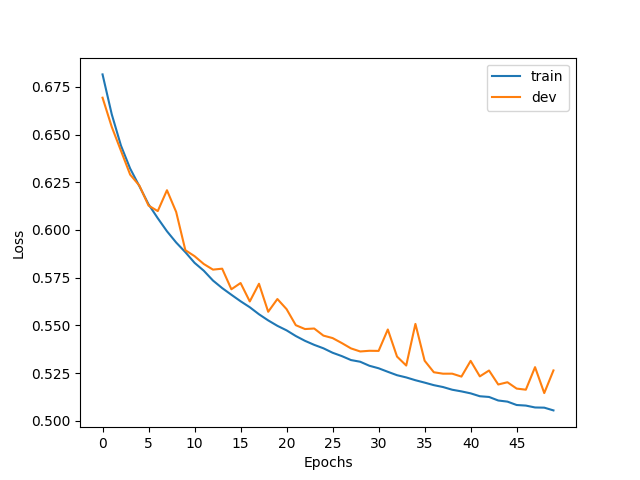
\includegraphics[width=0.45\textwidth]{gradient_descent_loss.png}
    \caption{train and dev loss}
\end{figure}\\


\bibliographystyle{apalike}
\bibliography{ref}

\end{document}